\chapter{Failure Modes}
\label{chp:failure-modes}

In this chapter we will discuss different ways the protocol might fail, or situations that might compromise the integrity of the communication.

\section{Key Loss}\label{sec:key-loss}

If the secret key K is compromised you have a short window wherein you might trigger a re-keying of the satellite, comparable to how you would handle a lost password. The re-keying involves running a authenticated \gls{dh} key exchange, after completing the two-way authentication in the protocol. If the attacker who got possession of the secret key does this before you, you'll have lost your satellite. How to avoid securely store and handle keys is outside the scope of this paper, but anyone handling the master keys should be trained in managing sensitive data.

To mitigate the consequences of a master key loss, a key hierarchy should be used, where some keys can be used for operational purposes like taking pictures, and reading sensor data, while a more heavily guarded key can be used for mission-critical operations such as code upload, setting satellite orientation, resetting subsystems, re-keying, etc.

If a session key is lost, the potential consequences depend on whether a key hierarchy have been implemented or not. If role-based access control is implemented and the session key is unprivileged (i.e. can not perform a master re-key) it doesn't affect any of the other running session, previous or upcoming, as the session key is only dependent on \( R_a \) and \( R_b \) and the shared secret, and not on any previous keys. If it's an unprivileged session and you still have the key, you'd send a \texttt{CLIENT\_TERMINATE} for the server to quit the session and invalidate the session key. If you've lost the session key, you should start a new one with a privileged key and run a re-key to invalidate all existing sessions. If the session is privileged it's equivalent to loosing the master key, and your handling of the issue should be the same. This is why more work into separating normal usage from administrative use like re-keying should be done, with e. g. role based access, as briefly discussed in \autoref{sec:extension-points}.


\section{Invalid MAC Computations}\label{sec:invalid-mac}

If the server or client receives a message with an invalid MAC there's a couple of different things that could have caused this:

\begin{itemize}
    \item Message corruption not detected by the CRC32 on the underlying layer
    \item Client failed to use the correct MAC function as negotiated during the handshake, or derived a faulty session key
    \item Someone is sending bogus messages without knowing the secret key and/or the protocol
\end{itemize}

In all cases, the server should simply ignore the message as it has no way to differentiate the different situations. All of these can also occur on the client side, and the mitigation is the same, ignore the message and wait for one with a valid MAC.


\section{RNG Failure}\label{sec:rng-failure}

Much of the security of the protocol hinges on the strength of the random number generators on both sides of the communication. However, the most crucial one is the one residing on the satellite side. If the client has a faulty RNG and sends the same \( R_b \) twice, he has no guarantees that the reply comes from the actual satellite, as an attacker might have intercepted a valid reply to this challenge previously, and can respond with the same \( R_a \) and thus the same signature that the legitimate satellite used last time this \( R_b \) was used. The session key derived would be the same as last time, since the session key only depends on the shared key, \( R_a \) and \( R_b \). The attacker won't know the actual session key, but would be able to replay the satellite messages from the previous session.

If the satellite were to re-use a previous \( R_a \), you'd get a similar but mirrored attack vector. An attacker could re-send a previously sent \( R_b \) with a valid signature, get the same response from the satellite as last time, which means that the session key will be the same. He can now replay all the messages the client sent in the previous session. The attacker can not change the master key in this attack, since the key exchange involves a secret part not sent in the clear, without which the attacker would not be able to derive the new key, or confirm the key exchange, since the satellite will require a confirmation on the new key before completing the change.


\section{Replay Attacks}\label{sec:replay-attacks}

The only way for someone not knowing the shared secret to get any interaction with the satellite is to replay a previously sent message by a legitimate client. If a previous CLIENT\_HELLO is replayed, the attacker will get a valid reply from the server, but will be unable to generate a valid signature for the SA\_PROPOSAL message that should follow.

If the attacker tries to replay a CLIENT\_DATA message, as long as the satellite has received the message previously it will discard the message since the sequence number doesn't match what the satellite is expecting.

If the server hasn't processed the message yet, there's a possibility the attacker could affect the application. This could happen if the client sends a valid message, but the server is being jammed by an attacker that also intercepts the client's message. The attacker could now be the first one to send the message, and could get a reply from the server. He could also jam the client, keeping the client in the dark about the server's response to the attacker's message. However, the message will be one the client intended to send in the first place, but could be time-shifted by the attacker. Assuming the presence of a clock on both sides, an application could mitigate this by adding timestamps to timing-critical messages, and thus rejecting out of date messages. Each application protocol would need to specify their requirements in terms of clock accuracy and allowed window of execution.

No mitigation for this attack will be included in the proposed protocol, as we consider it to be the responsibility of the application-layer protocol to do a risk-assessment of whether this is something worth mitigating. Note also that if the client sends another command that is received by the server, it will invalidate the attacker's message. This works since the server now expects a sequence number great than the one that's in the message the attacker possesses.


\section{Denial of Service}

It's hard to prevent \acrfull{dos} for a service running over a radio interface, since it's a shared medium and it only requires one person to fully jam the interface for all other participants. This is in contrast to the wired Internet, where the backbone has vastly more capacity than what any single user has through her connection, and thus any effective \gls{dos} on the Internet has to be a \emph{Distributed} DoS (DDoS), where several users team up to join the strength of their connections. The users behind the connections might be unaware of the attack, as they might have had their computers get infected by a virus, and is part of botnet.

Migrations for DDoS is to some extent possible on the Internet though, since many attacks rely on spoofing the source IP. The service can thus verify that there's an actual user behind that IP, by issuing a challenge that needs to be responded to before the server will invest any resources in answering the request.

This mitigation technique is not possible over a radio link though, since there's no routing and anyone can claim any address they want. Thus, if an attacker captures a valid $R_b$ and \( MAC_k(R_b) \) pair, he can issue this from several addresses to force the server into verifying the MAC for all of the requests, generate an $R_a$ and allocate a session. The attacker will be unable to send any more messages to any of the sessions, but can create as many sessions as he desires, and thus potentially exhausting the memory of the server. The mitigation for this is to have low timeout values for the handshake messages, and longer timeouts for established sessions. This makes sure that the server discards the stuck-in-handshake sessions faster than the attacker can create them.

Timeout values would need to be configured for each underlying transport, for UDP-based environments one second (or potentially even lower) timeout should be enough to allow legitimate requests to establish a session without troubles. The same timeout value -- or slightly higher, to allow more room for the public-key cryptography -- is recommended for the re-key related messages as well. How long established sessions can stay alive without a heartbeat can easily be several hours or even days or weeks, as long as the server has enough memory to store the state of all the sessions that might appear over the period.


\section{Power Analysis}

\begin{figure}[ht!]
\centering
    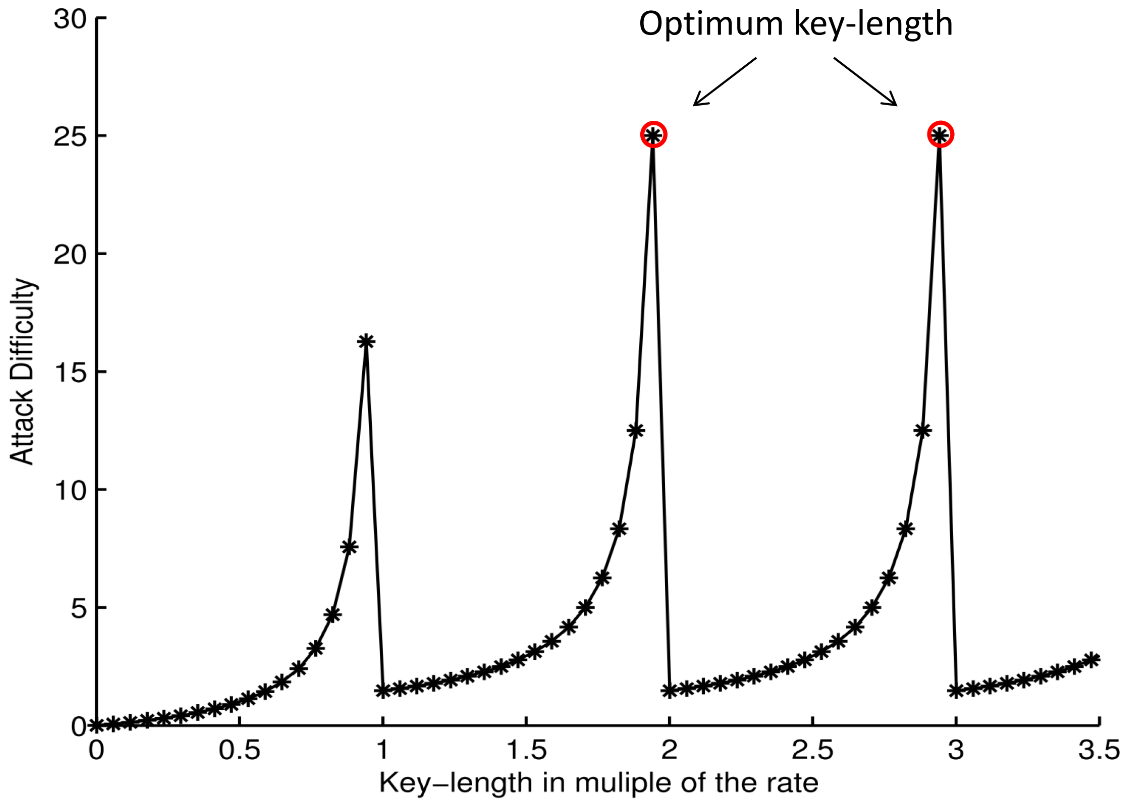
\includegraphics[width=110mm]{optimum-key-length}
    \caption{Optimal key lengths for MAC-Keccak. Illustration by Taha and Schaumont (\cite{keccak_side_channel_analysis})}\label{fig:optimum-key-length}
\end{figure}

Taha and Schaumont performed a side-channel analysis of MAC-Keccak in 2013 \cite{keccak_side_channel_analysis}, concluding with a recommended key size of \( 2*rate-1 \) to make side-channel analysis as costly as possible. The relationship between key size and cost of performing a side-channel attack is depicted in \autoref{fig:optimum-key-length}. This implies that the optimum key size for MAC-Keccak is 2175 and 1023 bits, for Keccak-256 and Keccak-512 respectively. These key sizes are significantly larger than the ones we're using in NAP, which means that a side-channel attack against the protocol using power analysis might reveal the key used for MAC computation if a sufficient amount of power traces are acquired. From the analysis by Taha and Schaumont, 5000 power traces yielded close to 90\% chance of recovering 320-bit keys against MAC-Keccak with rate 1088. Thus we can only assume that recovering our 128-bit session keys requires far fewer traces.

We're not trying to mitigate side-channel attacks in this version of the protocol, partly due to the increased storage cost of bumping the key size, and that the attack can be mitigated by physically securing the computers of the communicating parties. If a deployment of \gls{nap} can not physically secure the communicating computers, the attack can be made costlier by implementing a version of \gls{nap} with larger key sizes.

Using power analysis it's also possible to perform a timing attack against the MAC check against a naïve implementation, if the implementation does a direct string comparison of the expected MAC and the given MAC. The fault here lies in the fact that the naïve comparison will terminate on the first differing byte, thus leaking key-related data onto a side channel (time). The attacker could then guess on the first byte of the MAC, and the power analysis will reveal a slightly earlier return to idle if the guess was wrong, compared to if it was right. Thus, in 256 guesses he'd know the first correct byte of the MAC for his message. He can now continue on to the next byte, completing the entire MAC in \( 256 \times 8 = 2048 \) guesses. The sample implementation is not vulnerable to this attack, as it uses a constant-time comparison of the MACs. Note that this attack is not feasible without the power traces, as NAP doesn't give any reply to MAC failures, and thus it's not possible to profile the different guesses.
